% !TEX program = xelatex
% =====================================================================
%  note.tex  --  a single note (one file per topic).
%  Copy this file to start a new note; replace the \input lines with
%  your own content.
% =====================================================================
\documentclass[11pt]{article}
\usepackage{mynotes}
\notesetup{Short Title}{Author Name}{https://example.com}  % header, footer, link
% \showsolutionsfalse   % hide all solutions (e.g. for a handout)

\begin{document}
\notetitle{Title of the Note}

% ---------------------------------------------------------------------
%  Sample content: text, lists and mathematics
% ---------------------------------------------------------------------
\section{Text and lists}\label{sec:text}

This document is a sample built with the template. Each section shows one
kind of element, so you can see the final look before writing your own notes.
Replace this text with your content.

Body text supports \emph{emphasis}, \textbf{bold text},
\hl{highlighted key terms}, inline code such as \code{result = compute(data)},
and links such as \href{https://example.com}{example.com}.\footnote{Footnotes
appear at the bottom of the page.}

\begin{itemize}
  \item Bullet lists use the accent color.
  \item They can be nested:
  \begin{itemize}
    \item a second-level item
    \item another second-level item
  \end{itemize}
  \item[\textcolor{co-green}{\checkmark}] Custom markers are possible too.
\end{itemize}

\begin{enumerate}
  \item Numbered lists
  \item keep the spacing compact
  \item and align neatly.
\end{enumerate}

\subsection{A subsection}

Subsections and subsubsections share the accent color, with smaller sizes.
The header of each page shows the current section.

\subsubsection{A subsubsection}

Paragraphs are separated by a small gap instead of an indent, which keeps
notes easy to scan.

% ---------------------------------------------------------------------
\section{Mathematics}\label{sec:math}

Inline math sits in the text: $f\colon \R^n \to \R$, $\norm{\vect{x}}$,
$\abs{a - b}$ and $\inner{\vect{u}}{\vect{v}}$. Letters and digits use the same
typeface as the text.

A numbered equation can be referenced later:
\begin{equation}\label{eq:sample}
  \int_a^b f(x)\,dx = F(b) - F(a).
\end{equation}

A multi-line derivation, aligned at the equals sign, with only the last line
numbered:
\begin{align}
  (a + b)^2 &= (a + b)(a + b) \nonumber\\
            &= a^2 + 2ab + b^2. \label{eq:aligned}
\end{align}

Matrices, sums, fractions and cases:
\[
  A = \begin{bmatrix} a_{11} & a_{12} \\ a_{21} & a_{22} \end{bmatrix},
  \qquad
  \sum_{k=1}^{n} k = \frac{n(n+1)}{2},
  \qquad
  \abs{x} = \begin{cases} x, & x \ge 0, \\ -x, & x < 0. \end{cases}
\]
References such as \eqref{eq:sample} and \eqref{eq:aligned} are clickable links.
       % text, lists, mathematics
% ---------------------------------------------------------------------
%  Sample content: numbered boxes
% ---------------------------------------------------------------------
\section{Numbered boxes}\label{sec:boxes}

Numbered boxes hold the content you will refer back to. Each one takes an
optional title and an optional label; the number follows the section.

\begin{definition}[Title of the definition][def:sample]
A \emph{definition} states precisely what a term means. For example, a
function $f$ is \emph{increasing} if $x < y$ implies $f(x) \le f(y)$.
\end{definition}

\begin{theorem}[Title of the theorem][thm:sample]
A \emph{theorem} states a main result. If $f$ and $g$ are increasing, then
$f + g$ is increasing.
\end{theorem}

\begin{proof}
Let $x < y$. By \cref{def:sample}, $f(x) \le f(y)$ and $g(x) \le g(y)$.
Adding the two inequalities gives $(f + g)(x) \le (f + g)(y)$.
\end{proof}

\begin{lemma}
Lemmas, propositions and corollaries share the color and the counter of
theorems.
\end{lemma}

\begin{corollary}
By \cref{thm:sample}, any finite sum of increasing functions is increasing.
\end{corollary}

\begin{example}[][ex:sample]
Examples are shown in blue. Both $f(x) = x$ and $g(x) = x^3$ are increasing,
so $x + x^3$ is increasing as well.
\end{example}

\begin{remark}
Remarks are gray, for side comments that do not need emphasis.
\end{remark}

\begin{exercise}[][exer:sample]
Exercises are orange. Show that $h(x) = -x$ is not increasing.
\end{exercise}

\begin{solution}
Take $x = 0 < 1 = y$. Then $h(0) = 0 > -1 = h(1)$. Solutions can be hidden
for handouts with \code{\showsolutionsfalse}.
\end{solution}
      % definition, theorem, proof, example, ...
% ---------------------------------------------------------------------
%  Sample content: callouts
% ---------------------------------------------------------------------
\section{Callouts}\label{sec:callouts}

Callouts are unnumbered side notes. Each type has its own color and icon, and
any of them accepts a custom title in brackets.

\begin{note}
Use a note for extra context the reader may find useful.
\end{note}

\begin{info}
Use info for background information or a quick fact.
\end{info}

\begin{tip}[A custom title]
This tip has a custom title instead of the default one.
\end{tip}

\begin{important}
Use important for something the reader should not skip.
\end{important}

\begin{summary}
Use a summary to wrap up a section in one or two sentences.
\end{summary}

\begin{success}
Use success for a confirmed result or a check that passed.
\end{success}

\begin{question}
Use a question to make the reader think before reading on.
\end{question}

\begin{warning}
Use a warning for a common mistake or a condition that must hold.
\end{warning}

\begin{failure}
Use failure for an approach that does not work, and why.
\end{failure}

\begin{danger}
Use danger for a step that can cause serious errors.
\end{danger}

\begin{bug}
Use bug for a known issue or a correction.
\end{bug}

\begin{todo}
Use todo for a reminder of work still to be done.
\end{todo}

\begin{quotebox}[Author of the quote]
A quotation, with its source as the title.
\end{quotebox}

The types \code{hint}, \code{tldr}, \code{faq}, \code{caution} and
\code{attention} are also available, and new ones can be defined with
\code{\newcallout}.
   % note, tip, warning, ...
% ---------------------------------------------------------------------
%  Sample content: code, tables, figures and algorithms
% ---------------------------------------------------------------------
\section{Code}\label{sec:code}

A whole source file, with line numbers and the file name as the title:

\pyfile{code/example.py}

Program output in a terminal block:

\begin{terminal}
$ python code/example.py
mean = 5.00, std = 2.00
\end{terminal}

Any language supported by the \code{listings} package:

\begin{codeblock}{C++}[main.cpp]
#include <iostream>

int main() {
    std::cout << "Hello, world!" << std::endl;
    return 0;
}
\end{codeblock}

% ---------------------------------------------------------------------
\section{Tables and figures}\label{sec:tables}

Tables and figures stay exactly where they are written. The first row of a
table is the header; the rows below it are striped automatically.

\begin{datatable}[A striped table][tab:sample]{lccr}
\thead{Item} & \thead{Group} & \thead{Status} & \thead{Value} \\
\midrule
Alpha & A & done & 12.5 \\
Beta  & A & open &  8.0 \\
Gamma & B & done & 15.2 \\
Delta & B & open &  4.7
\end{datatable}

\begin{widetable}[A full-width table with wrapping text][tab:wide]{lLl}
\thead{Element} & \thead{Description} & \thead{Example} \\
\midrule
Box     & Numbered content with an optional title and a label for references. & \code{theorem} \\
Callout & Unnumbered side note with an icon, in one of six colors.            & \code{warning} \\
Code    & Highlighted source code with line numbers and a file name.          & \code{python}
\end{widetable}

\begin{notefigure}[A plot drawn with pgfplots][fig:plot]
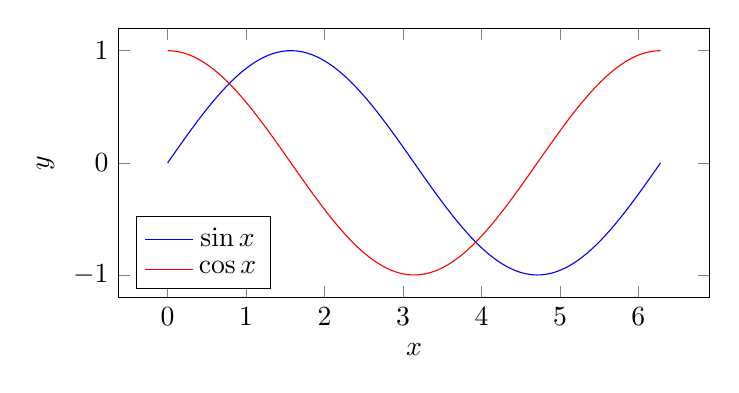
\begin{tikzpicture}
\begin{axis}[width=0.75\linewidth, height=5cm, xlabel={$x$}, ylabel={$y$},
             domain=0:6.283, samples=100, legend pos=south west]
  \addplot+[no marks] {sin(deg(x))};
  \addplot+[no marks] {cos(deg(x))};
  \legend{$\sin x$, $\cos x$}
\end{axis}
\end{tikzpicture}
\end{notefigure}

\begin{notefigure}[Images from files, side by side][fig:images]
  \begin{subfigure}{0.32\linewidth}\centering
    \includegraphics[width=\linewidth]{example-image-a}\caption{First image}
  \end{subfigure}\quad
  \begin{subfigure}{0.32\linewidth}\centering
    \includegraphics[width=\linewidth]{example-image-b}\caption{Second image}
  \end{subfigure}
\end{notefigure}

% ---------------------------------------------------------------------
\section{Algorithms}\label{sec:algorithms}

\begin{algorithm}[H]
\caption{A generic iterative procedure}\label{alg:sample}
\begin{algorithmic}[1]
\Require input data $D$, tolerance $\varepsilon > 0$
\Ensure result $r$
\State $r \gets$ initial guess
\Repeat
  \For{each item $d \in D$}
    \State update $r$ using $d$
  \EndFor
\Until{the change in $r$ is smaller than $\varepsilon$}
\State \Return $r$
\end{algorithmic}
\end{algorithm}

% ---------------------------------------------------------------------
\section{Cross-references}\label{sec:refs}

Every labeled element can be referenced by name and number, and each
reference is a link: \cref{def:sample}, \cref{thm:sample}, \cref{ex:sample},
\cref{eq:sample}, \cref{tab:sample}, \cref{fig:plot}, \cref{alg:sample} and
\cref{sec:math}.

\begin{summary}
One style for notes, books and slides. Replace the sample content with your
own and keep the structure.
\end{summary}
       % code, tables, figures, algorithms, references
\end{document}
